% Shared style for all Git & GitHub lectures (same look as the N-body course)
\documentclass[11pt,a4paper]{article}
\usepackage[margin=2.3cm]{geometry}
\usepackage[T1]{fontenc}
\usepackage{lmodern}
\usepackage{upquote}   % straight quotes in monospaced text, so commands can be copied
\usepackage{microtype}
% keep '--' as two real hyphens in monospace text (commands like --version)
\DisableLigatures[-,<,>]{family=tt*}
\usepackage{booktabs,enumitem,graphicx,xcolor}
\usepackage{array}
\usepackage{needspace}
\usepackage{longtable}
\usepackage{float}
\usepackage{tikz}
\usetikzlibrary{arrows.meta,calc,positioning,decorations.pathreplacing,shapes.geometric,fit,backgrounds}
\usepackage[most]{tcolorbox}
\usepackage{listings}
\usepackage{fancyhdr}
\usepackage[colorlinks=true,linkcolor=blue!50!black,urlcolor=blue!50!black,citecolor=blue!50!black]{hyperref}

\setlength{\parindent}{0pt}
\setlength{\parskip}{0.6em}
\setlength{\abovecaptionskip}{4pt}
\usepackage[font=small,labelfont=bf]{caption}
\setlist{itemsep=0.2em,topsep=0.3em}

% ---------- colours ----------
\definecolor{cbg}{HTML}{F6F8FA}
\definecolor{ckw}{HTML}{0B5CAD}
\definecolor{ccm}{HTML}{6A737D}
\definecolor{cst}{HTML}{B5451B}
\definecolor{cpart}{HTML}{1F6FB2}
\definecolor{cheavy}{HTML}{C0392B}
\definecolor{cgreen}{HTML}{2E8B57}

% ---------- terminal listings ----------
% In a terminal session, lines starting with "$" are what YOU type.
% Everything else is what Git prints back.
\lstdefinestyle{term}{
  basicstyle=\ttfamily\small, backgroundcolor=\color{cbg},
  frame=single, rulecolor=\color{black!15}, showstringspaces=false,
  breaklines=true, columns=fullflexible, keepspaces=true,
  aboveskip=0.6em, belowskip=0.6em, xleftmargin=4pt, xrightmargin=4pt,
  literate={\$\ }{{\textcolor{cgreen}{\$\ }}}2,
  upquote=true
}
\lstset{style=term}
\newcommand{\code}[1]{\texttt{\small #1}}

% ---------- boxes ----------
\newtcolorbox{history}{colback=yellow!8,colframe=orange!60!black,
  title={History},fonttitle=\bfseries\small,left=4pt,right=4pt,top=2pt,bottom=2pt}
\newtcolorbox{quickfact}{colback=purple!4,colframe=purple!55!black,
  title={Quick fact},fonttitle=\bfseries\small,left=4pt,right=4pt,top=2pt,bottom=2pt}
\newtcolorbox{keyidea}{colback=blue!4,colframe=blue!50!black,
  title={Key idea},fonttitle=\bfseries\small,left=4pt,right=4pt,top=2pt,bottom=2pt}
\newtcolorbox{pitfall}{colback=red!4,colframe=red!55!black,
  title={Pitfall},fonttitle=\bfseries\small,left=4pt,right=4pt,top=2pt,bottom=2pt}
\newtcolorbox{tryit}{colback=teal!5,colframe=teal!55!black,
  title={Try it},fonttitle=\bfseries\small,left=4pt,right=4pt,top=2pt,bottom=2pt,breakable}
\newtcolorbox{homework}[1]{colback=green!4,colframe=green!40!black,
  title={Homework #1},fonttitle=\bfseries\small,left=4pt,right=4pt,top=2pt,bottom=2pt,
  breakable}
\newtcolorbox{goals}{colback=gray!6,colframe=gray!60!black,
  title={Learning goals},fonttitle=\bfseries\small,left=4pt,right=4pt,top=2pt,bottom=2pt}

% Solutions always start on a fresh page, behind a clear warning.
\newcommand{\solutionspage}{%
  \clearpage
  \begin{tcolorbox}[colback=red!6,colframe=red!60!black,halign=center]
    {\Large\bfseries Solutions}\\[0.3em]
    {\small Stop here if you have not tried the homework yet.\\
    Attempt every task first, run the checker, and only then read on.}
  \end{tcolorbox}
}

% ---------- Git diagram styles (TikZ) ----------
\tikzset{
  commit/.style={circle,draw=black!70,fill=blue!10,minimum size=7mm,inner sep=0pt,font=\scriptsize\ttfamily},
  newcommit/.style={commit,fill=orange!25,dashed},
  tag/.style={draw,rounded corners=2pt,font=\scriptsize\ttfamily,inner sep=2pt},
  branchtag/.style={tag,fill=green!15,draw=green!40!black},
  headtag/.style={tag,fill=yellow!30,draw=orange!70!black},
  remotetag/.style={tag,fill=purple!10,draw=purple!60!black},
  area/.style={draw,rounded corners,minimum height=11mm,minimum width=33mm,align=center,font=\small},
  cmdarrow/.style={->,thick,>=Stealth},
  link/.style={->,thick,>=Stealth,black!70},
}

% ---------- header ----------
\pagestyle{fancy}
\fancyhf{}
\renewcommand{\headrulewidth}{0.3pt}
\fancyfoot[C]{\thepage}
\newcommand{\lecturetitle}[3]{%
  \fancyhead[L]{\small\textit{Git \& GitHub from Zero}}
  \fancyhead[R]{\small Lecture #1}
  \begin{center}
    {\Large\bfseries Lecture #1}\\[0.4em]
    {\LARGE\bfseries #2}\\[0.4em]
    {\small #3}
  \end{center}
  \vspace{0.5em}
}

\begin{document}
\lecturetitle{3}{Reading History and Undoing Mistakes}{\texttt{log}, \texttt{show}, \texttt{diff}, \texttt{restore}, \texttt{commit --amend}, and \texttt{revert}}

\begin{goals}
\begin{itemize}
  \item Read the history of a project with \code{git log} and \code{git show}, and name commits with \code{HEAD} and \code{HEAD\textasciitilde{}n}.
  \item Compare versions with the three forms of \code{git diff}, and read a diff.
  \item Undo a mistake at the right stage: unstage, discard, amend, or revert.
  \item Tell \emph{safe} undo commands from commands that destroy work.
\end{itemize}
\end{goals}

\section{Why this lecture matters}

Version control earns its keep when something goes wrong. Everyone saves the wrong file, mistypes a message, or deletes a line they needed. Git gives you a tool for each situation, but the tools differ in one crucial way: some are completely safe, and one throws work away for good. Learning which is which turns Git from scary into reassuring.

We will use a small practice repository whose history is the same on every computer. From the course folder run:

\begin{lstlisting}
$ bash codeHints/L03/setup_demo3.sh
$ cd practice/demo3
\end{lstlisting}

It creates \code{demo3} with four commits (a README and three recipes). Commit IDs are computed from the content, author and date, and the script fixes all of these, so the IDs printed in this lecture are the ones you will see. (On Windows with automatic line-ending conversion they may differ; everything else still works. If you ever want a fresh copy, add \code{--reset}.)

\section{Reading the history}

\subsection{\texttt{git log}}

\begin{lstlisting}
$ git log
commit 659ed06370bf2b80289ead79663c5ce21ba67c61
Author: Practice User <practice@example.com>
Date:   Mon Mar 4 09:00:00 2024 +0000

    Add waffle recipe

commit c595297a5267368106009265a473686c8d8ec827
Author: Practice User <practice@example.com>
Date:   Sun Mar 3 09:00:00 2024 +0000

    Add crepe recipe
...
\end{lstlisting}

The newest commit comes first. Each entry shows the full 40-character ID, the author, the date and the message. If the output is longer than the screen, Git shows it in a \emph{pager}: scroll with the arrow keys or space, and press \code{q} to quit.

Usually the compact form is enough:

\begin{lstlisting}
$ git log --oneline
659ed06 Add waffle recipe
c595297 Add crepe recipe
906ca29 Add pancake recipe
9d99f7a Add README
\end{lstlisting}

A few useful options (they can be combined):

\begin{center}
\small
\begin{tabular}{@{}l >{\raggedright\arraybackslash}p{9.4cm}@{}}
\toprule
Command & What it shows \\
\midrule
\code{git log --oneline} & One line per commit: short ID and message. \\
\code{git log -n 2} & Only the 2 newest commits (also works as \code{-2}). \\
\code{git log --stat} & Also which files each commit changed, with counts of added and removed lines. \\
\code{git log --grep=crepe} & Only commits whose message contains the word. \\
\code{git log --oneline --graph} & Draws the shape of the history. With one straight line it is not exciting; it becomes useful with branches in Lecture 4. \\
\bottomrule
\end{tabular}
\end{center}

\subsection{\texttt{git show}: one commit in detail}

\begin{lstlisting}
$ git show HEAD
commit 659ed06370bf2b80289ead79663c5ce21ba67c61
Author: Practice User <practice@example.com>
Date:   Mon Mar 4 09:00:00 2024 +0000

    Add waffle recipe

diff --git a/recipes.txt b/recipes.txt
index 2d1a741..0104975 100644
--- a/recipes.txt
+++ b/recipes.txt
@@ -1,2 +1,3 @@
 Pancakes: flour, milk, eggs
 Crepes: flour, milk, eggs, butter
+Waffles: flour, milk, eggs, sugar
\end{lstlisting}

\code{git show} prints the message and then the \emph{change} the commit made (a ``diff'', explained below). You can give it any commit ID: \code{git show c595297}. The short 7-character ID is enough as long as it is unambiguous.

\subsection{Naming commits: \texttt{HEAD}, \texttt{HEAD\textasciitilde{}1}}

You rarely want to copy IDs. Git has names for commits relative to where you are:

\begin{figure}[H]
\centering
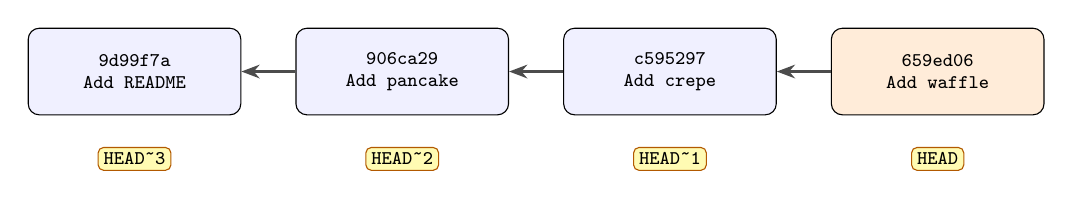
\begin{tikzpicture}[
  cb/.style={draw,rounded corners,fill=blue!6,minimum width=2.7cm,minimum height=11mm,align=center,font=\scriptsize\ttfamily,inner sep=3pt},
  nm/.style={tag,fill=yellow!30,draw=orange!70!black}]
  \node[cb] (a) at (0,0)   {9d99f7a\\Add README};
  \node[cb] (b) at (3.4,0) {906ca29\\Add pancake};
  \node[cb] (c) at (6.8,0) {c595297\\Add crepe};
  \node[cb,fill=orange!15] (d) at (10.2,0) {659ed06\\Add waffle};
  \draw[link] (b)--(a); \draw[link] (c)--(b); \draw[link] (d)--(c);
  \node[nm,below=4mm of d] {HEAD};
  \node[nm,below=4mm of c] {HEAD\textasciitilde{}1};
  \node[nm,below=4mm of b] {HEAD\textasciitilde{}2};
  \node[nm,below=4mm of a] {HEAD\textasciitilde{}3};
\end{tikzpicture}
\caption{\code{HEAD} is the commit you are currently on (the newest one, for now). \code{HEAD\textasciitilde{}1} is its parent, \code{HEAD\textasciitilde{}2} its grandparent, and so on. Arrows point from a commit to its parent.}
\label{fig:head}
\end{figure}

So \code{git show HEAD\textasciitilde{}1} shows the crepe commit. You will use \code{HEAD} constantly: it means ``where I am now''.

\begin{tryit}
In \code{demo3}, run \code{git log --oneline}, then \code{git show HEAD\textasciitilde{}2}, then \code{git log --stat -n 2}. Which file did the very first commit create? (Use \code{git show 9d99f7a}.)
\end{tryit}

\section{Comparing versions: \texttt{git diff}}

A \textbf{diff} lists the differences between two versions. Remember the three areas from Lecture 2: \code{git diff} compares different pairs of them.

\begin{figure}[H]
\centering
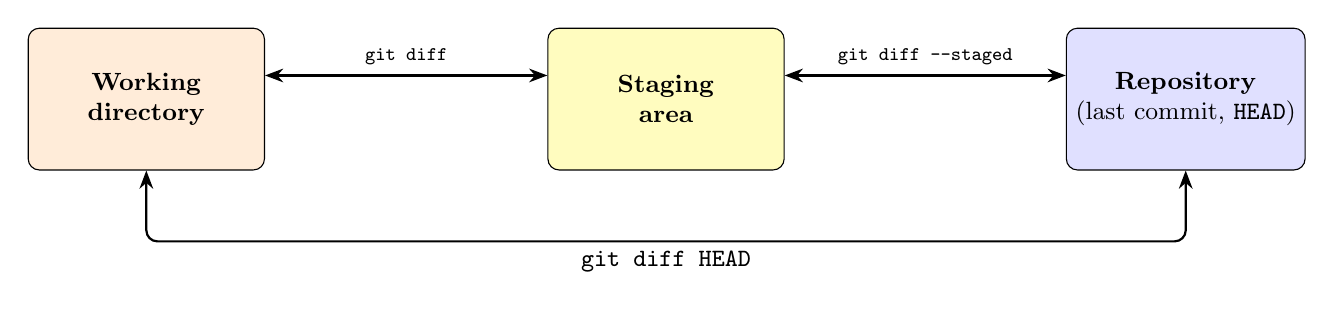
\begin{tikzpicture}
  \node[area,fill=orange!15,minimum width=30mm,minimum height=18mm] (wd) at (0,0) {\textbf{Working}\\\textbf{directory}};
  \node[area,fill=yellow!25,minimum width=30mm,minimum height=18mm] (st) at (6.6,0) {\textbf{Staging}\\\textbf{area}};
  \node[area,fill=blue!12,minimum width=30mm,minimum height=18mm] (re) at (13.2,0) {\textbf{Repository}\\(last commit, \code{HEAD})};
  \draw[<->,thick,>=Stealth] ([yshift=3mm]wd.east) -- node[above,font=\scriptsize\ttfamily] {git diff} ([yshift=3mm]st.west);
  \draw[<->,thick,>=Stealth] ([yshift=3mm]st.east) -- node[above,font=\scriptsize\ttfamily] {git diff --staged} ([yshift=3mm]re.west);
  \draw[<->,thick,>=Stealth,rounded corners] (wd.south) -- ++(0,-0.9) -- node[below,font=\small\ttfamily] {git diff HEAD} ($(re.south)+(0,-0.9)$) -- (re.south);
\end{tikzpicture}
\caption{Which areas each form of \code{git diff} compares.}
\label{fig:diff}
\end{figure}

Make a change to see them in action:

\begin{lstlisting}
$ echo "Muffins: flour, milk" >> recipes.txt
$ git diff
diff --git a/recipes.txt b/recipes.txt
index 0104975..11161ec 100644
--- a/recipes.txt
+++ b/recipes.txt
@@ -1,3 +1,4 @@
 Pancakes: flour, milk, eggs
 Crepes: flour, milk, eggs, butter
 Waffles: flour, milk, eggs, sugar
+Muffins: flour, milk
\end{lstlisting}

\textbf{Reading a diff.}
\begin{itemize}
  \item \code{--- a/recipes.txt} is the old version, \code{+++ b/recipes.txt} the new one.
  \item A line starting with \code{+} was \emph{added}; a line starting with \code{-} was \emph{removed}; lines with a space in front are unchanged context, shown to help you find your place.
  \item \code{@@ -1,3 +1,4 @@} says: this block (a \emph{hunk}) covers lines 1--3 of the old file and lines 1--4 of the new one.
  \item (The \code{index} line holds internal IDs; you can ignore it.)
\end{itemize}

Now stage the change and look again:

\begin{lstlisting}
$ git add recipes.txt
$ git diff                    # prints nothing: working dir == staging area
$ git diff --staged           # staging area vs last commit
diff --git a/recipes.txt b/recipes.txt
...
+Muffins: flour, milk
\end{lstlisting}

\begin{center}
\small
\begin{tabular}{@{}l >{\raggedright\arraybackslash}p{9.0cm}@{}}
\toprule
Command & Compares \\
\midrule
\code{git diff} & Working directory \emph{against} the staging area: changes you have \emph{not yet staged}. \\
\code{git diff --staged} & Staging area against the last commit: what the next commit \emph{would contain}. \\
\code{git diff HEAD} & Working directory against the last commit: \emph{everything} changed since then. \\
\code{git diff A B} & Two commits, e.g. \code{git diff HEAD\textasciitilde{}2 HEAD}. \\
\code{git diff --stat} & (add to any of the above) Only a summary of files and line counts. \\
\bottomrule
\end{tabular}
\end{center}

\begin{keyidea}
Run \code{git diff --staged} before every commit to check exactly what you are about to save. It is the best habit in this whole course.
\end{keyidea}

\begin{pitfall}
An empty \code{git diff} does not mean ``nothing changed''. It means nothing changed \emph{that is not already staged}. If you just ran \code{git add}, look with \code{git diff --staged}.
\end{pitfall}

\section{Undoing mistakes}

Mistakes happen at different stages, and each stage has its own fix:

\begin{center}
\small
\begin{tabular}{@{}>{\raggedright\arraybackslash}p{4.7cm} >{\raggedright\arraybackslash}p{4.7cm} >{\raggedright\arraybackslash}p{3.6cm}@{}}
\toprule
The mistake is\ldots & Use & Safe? \\
\midrule
staged by accident & \code{git restore --staged file} & safe \\
edited, and you want the old text back & \code{git restore file} & \textbf{destroys your edit} \\
in the last commit (message or a forgotten file) & \code{git commit --amend} & rewrites that commit \\
in an older commit & \code{git revert commit} & safe \\
\bottomrule
\end{tabular}
\end{center}

We go through them one by one.

\subsection{Unstage: \texttt{git restore --staged}}

You staged a file you did not mean to. Unstaging moves it back to ``modified'' and \emph{keeps your edit}:

\begin{lstlisting}
$ git status --short
M  recipes.txt
$ git restore --staged recipes.txt
$ git status --short
 M recipes.txt
\end{lstlisting}

This is the command Git suggested in its status hints in Lecture 2. Nothing is lost.

\subsection{Discard: \texttt{git restore}}

\begin{pitfall}
\textbf{\code{git restore file} overwrites the file in your working directory with the last saved version. Your uncommitted edits are gone, and there is no undo}, because Git never saved them. Look first with \code{git diff file}, and only restore if you are sure.
\end{pitfall}

\begin{lstlisting}
$ git restore recipes.txt
$ git status --short
$ cat recipes.txt
Pancakes: flour, milk, eggs
Crepes: flour, milk, eggs, butter
Waffles: flour, milk, eggs, sugar
\end{lstlisting}

The status is empty (clean) and the Muffins line is gone for good. The same command can fetch an \emph{old} version of a file from any commit:

\begin{lstlisting}
$ git show HEAD~2:recipes.txt       # just look at the old version
Pancakes: flour, milk, eggs
$ git restore --source=HEAD~2 recipes.txt   # put it into the working directory
\end{lstlisting}

The second form also overwrites your current file, so it is a destructive step too (afterwards the file shows up as modified and you can commit it, or discard it again with plain \code{git restore}).

\subsection{Fix the last commit: \texttt{git commit --amend}}

You just committed and notice a typo in the message, or you forgot a file. \code{--amend} replaces the last commit with a corrected one:

\begin{lstlisting}
$ git commit --amend -m "Add waffles recipe (with sugar)"
[main f1c345f] Add waffles recipe (with sugar)
 Date: Mon Mar 4 09:00:00 2024 +0000
 1 file changed, 1 insertion(+)
\end{lstlisting}

(An amended commit gets an ID that depends on the moment you run the command, so yours will differ from \code{f1c345f}.)

To add a forgotten file to the last commit, stage it and amend while keeping the message:

\begin{lstlisting}
$ echo "Syrup: sugar, water" > syrup.txt
$ git add syrup.txt
$ git commit --amend --no-edit
\end{lstlisting}

\begin{figure}[H]
\centering
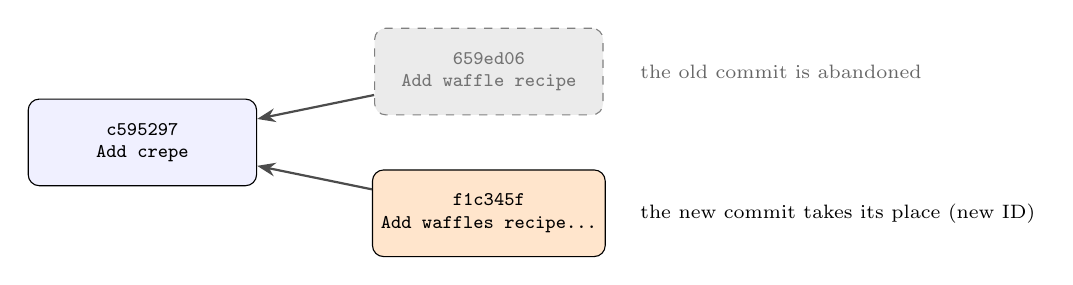
\begin{tikzpicture}[
  cb/.style={draw,rounded corners,minimum width=2.9cm,minimum height=11mm,align=center,font=\scriptsize\ttfamily,inner sep=3pt}]
  \node[cb,fill=blue!6] (p) at (0,0) {c595297\\Add crepe};
  \node[cb,fill=black!8,dashed,draw=black!50,text=black!55] (o) at (4.4,0.9) {659ed06\\Add waffle recipe};
  \node[cb,fill=orange!20] (n) at (4.4,-0.9) {f1c345f\\Add waffles recipe...};
  \draw[link] (o)--(p); \draw[link] (n)--(p);
  \node[font=\scriptsize,anchor=west,text=black!60] at (6.2,0.9) {the old commit is abandoned};
  \node[font=\scriptsize,anchor=west] at (6.2,-0.9) {the new commit takes its place (new ID)};
\end{tikzpicture}
\caption{Amending does not edit a commit, it \emph{replaces} it with a new one, which gets a new ID.}
\label{fig:amend}
\end{figure}

\begin{pitfall}
Amend only commits that nobody else has. Once you share a commit (Lecture 6 explains sharing), replacing it causes trouble for your collaborators. Rule: \textbf{amend only the most recent commit, and only if you have not shared it.} Otherwise use \code{revert}.
\end{pitfall}

\subsection{Undo an old commit safely: \texttt{git revert}}

\code{git revert} undoes a commit by making a \emph{new} commit that does the opposite. Nothing is erased, so it is always safe, even for shared work. (The listing below assumes a fresh \code{demo3}: run \code{setup\_demo3.sh --reset} first if you tried the amend examples. The new commit's ID depends on the time, so yours will differ from \code{02e79f4}.)

\begin{lstlisting}
$ git revert --no-edit HEAD
[main 02e79f4] Revert "Add waffle recipe"
 Date: Tue Mar 5 09:00:00 2024 +0000
 1 file changed, 1 deletion(-)
$ git log --oneline
02e79f4 Revert "Add waffle recipe"
659ed06 Add waffle recipe
c595297 Add crepe recipe
906ca29 Add pancake recipe
9d99f7a Add README
\end{lstlisting}

The waffle line is gone from \code{recipes.txt}, but the waffle commit is still in the history, followed by the commit that undoes it.

\begin{figure}[H]
\centering
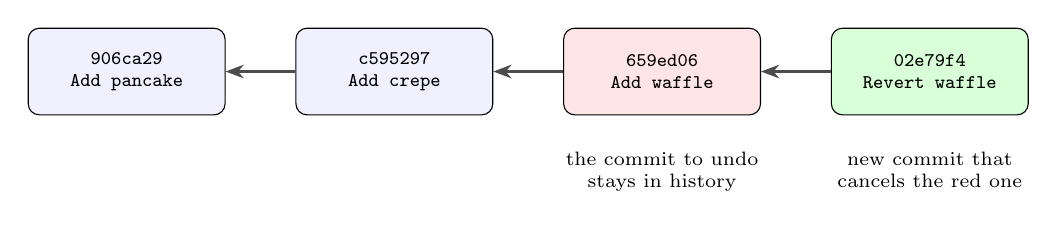
\begin{tikzpicture}[
  cb/.style={draw,rounded corners,minimum width=2.5cm,minimum height=11mm,align=center,font=\scriptsize\ttfamily,inner sep=3pt}]
  \node[cb,fill=blue!6] (a) at (0,0) {906ca29\\Add pancake};
  \node[cb,fill=blue!6] (b) at (3.4,0) {c595297\\Add crepe};
  \node[cb,fill=red!10] (c) at (6.8,0) {659ed06\\Add waffle};
  \node[cb,fill=green!15] (d) at (10.2,0) {02e79f4\\Revert waffle};
  \draw[link] (b)--(a); \draw[link] (c)--(b); \draw[link] (d)--(c);
  \node[font=\scriptsize,anchor=north,align=center] at (10.2,-0.9) {new commit that\\cancels the red one};
  \node[font=\scriptsize,anchor=north,align=center] at (6.8,-0.9) {the commit to undo\\stays in history};
\end{tikzpicture}
\caption{Revert adds to the history; it never removes anything. The project's \emph{contents} after the revert equal those after \code{c595297}.}
\label{fig:revert}
\end{figure}

By default \code{git revert} opens an editor for the message (the same vim trap as in Lecture 2); \code{--no-edit} accepts the standard message \code{Revert "..."}. You can revert any commit by ID. One caution: if later commits changed the same lines, Git cannot undo the old commit automatically and reports a \emph{conflict}. Here, reverting \code{c595297} would do that, because the waffle line sits right next to it. Run \code{git revert --abort} to cancel safely. Resolving conflicts is the subject of Lecture 5.

\subsection{Deleting and untracking files}

\begin{lstlisting}
$ git rm syrup.txt                # delete the file and stage the deletion
$ git rm --cached notes.txt       # stop tracking it, but keep the file on disk
\end{lstlisting}

\code{git rm file} removes the file from your folder and stages the removal; commit as usual. (Deleting by hand with your file manager works too: then \code{git add file} stages the deletion.) \code{git rm --cached} is the fix promised in Lecture 2 for a file that you committed by mistake and now want in \code{.gitignore}: Git forgets it but leaves it on disk. It remains in the old commits, so it is no cure for a leaked secret.

\section{Which tool when?}

\begin{keyidea}
Ask two questions. \emph{Is the mistake committed yet?} If not, use \code{restore} (and read the warning). \emph{If it is committed, is the commit shared?} If not, \code{--amend} is fine for the last one. If it may be shared, use \code{revert}.
\end{keyidea}

\begin{center}
\small
\begin{tabular}{@{}l l l@{}}
\toprule
Command & Changes\ldots & Can lose work? \\
\midrule
\code{git restore --staged f} & staging area & no \\
\code{git restore f} & working directory & \textbf{yes, permanently} \\
\code{git commit --amend} & replaces the last commit & old commit is abandoned \\
\code{git revert c} & adds a new commit & no \\
\bottomrule
\end{tabular}
\end{center}

(Lecture 10 shows how even ``abandoned'' commits can usually be rescued, and introduces \code{git reset}, a powerful tool we deliberately skip for now.)

\Needspace{12\baselineskip}
\section{Homework 3}

\begin{homework}{3: Rescue the repository}
From the course folder run:
\begin{lstlisting}
$ bash codeHints/L03/setup_hw3.sh
$ cd practice/hw3
\end{lstlisting}
You get a repository with four commits and a messy working directory. Run \code{git log --oneline}, \code{git status} and \code{git diff}/\code{git diff --staged} to see the situation: \code{list.txt} has a junk line that is not staged, and \code{notes.txt} has a change that is staged too early. Do the tasks in this order. If you get stuck or break something, rebuild with \code{bash codeHints/L03/setup\_hw3.sh --reset} (from the course folder).

\begin{description}[leftmargin=1.2em,style=nextline]
\item[3.1 Investigate] Using only \code{git log} (and \code{git show} if you like), find the ID of the commit whose message is \code{Buy fireworks} and the number of commits. In the file \code{practice/hw3\_answers.txt} (outside the repository) write two lines of the form
\begin{lstlisting}
fireworks=<7-character ID>
commits=<number>
\end{lstlisting}
\item[3.2 Discard the junk] Throw away the unwanted line in \code{list.txt} so the file matches the last commit again.
\item[3.3 Unstage] Take the change in \code{notes.txt} out of the staging area, but \emph{keep the edit} in the file. Afterwards \code{git status --short} should show \code{\ M notes.txt}.
\item[3.4 Fix the typo] The latest commit message says \code{Update notse}. Change it to \code{Update notes}. The \code{TODO: add syrup} line must \emph{not} end up in that commit.
\item[3.5 Revert] The fireworks were a bad idea. Undo the commit \code{Buy fireworks} with \code{git revert --no-edit}, using its ID from 3.1. History must keep growing, not shrink.
\item[3.6 Question] Add a third line to \code{practice/hw3\_answers.txt}: \code{no-undo=<command>}, naming the one Git subcommand from this lecture that can destroy uncommitted work with no way back.
\end{description}

The final state: five commits, a clean \code{list.txt}, and only \code{notes.txt} modified (not staged), still containing the TODO line.

\textbf{Check yourself:} from the course folder run \code{bash codeHints/L03/check\_hw3.sh}. All \code{PASS}, then compare with the solutions at the end of this lecture (or in \code{solutions/L03/}).
\end{homework}

\section{Summary}

\begin{itemize}
  \item \code{git log [--oneline]} lists history; \code{git show c} shows one commit; \code{HEAD}, \code{HEAD\textasciitilde{}1}\dots{} name commits relative to where you are.
  \item \code{git diff} (unstaged), \code{git diff --staged} (what you will commit), \code{git diff HEAD} (everything), \code{git diff A B} (two commits).
  \item Unstage with \code{restore --staged}; discard edits with \code{restore} (permanent!); fix the last unshared commit with \code{commit --amend}; undo an older commit safely with \code{revert}.
  \item \code{git rm} deletes and stages; \code{git rm --cached} untracks but keeps the file.
\end{itemize}

\textbf{Further reading:} \emph{Pro Git} (\url{https://git-scm.com/book}), Chapters 2.3 ``Viewing the Commit History'' and 2.4 ``Undoing Things''; \code{git help log}, \code{diff}, \code{restore}, \code{revert}.

\solutionspage

\section*{Solutions to Homework 3}

\begin{lstlisting}
$ bash codeHints/L03/setup_hw3.sh
$ cd practice/hw3
$ git log --oneline
e672c50 Update notse
6e1cc4f Buy fireworks
809893e Add recipe notes
2217470 Add shopping list
$ git restore list.txt
$ git restore --staged notes.txt
$ git commit --amend -m "Update notes"
$ git revert --no-edit 6e1cc4f
$ git status --short
 M notes.txt
$ printf 'fireworks=6e1cc4f\ncommits=4\nno-undo=restore\n' > ../hw3_answers.txt
\end{lstlisting}

(Your IDs for the first three commits match these because the setup script fixes author and dates. The amended and revert commits get new IDs.)

\textbf{3.1.} \code{git log --oneline} shows the ID \code{6e1cc4f} next to \code{Buy fireworks} and four lines, so \code{commits=4}. The answer file lives in \code{practice/}, outside the repository, so it does not show up as an untracked file.

\textbf{3.2.} \code{git diff list.txt} first shows the junk line \code{+oops delete me}. \code{git restore list.txt} removes it. This is the destructive command: it is correct here, because the line really was junk. You must do this \emph{before} the revert, because the revert changes \code{list.txt} too and Git will not overwrite your uncommitted edit.

\textbf{3.3.} \code{git restore --staged notes.txt} moves the \code{TODO: add syrup} line from ``staged'' back to ``modified''. The line stays in the file. Check with \code{git status --short}: the first column is now empty.

\textbf{3.4.} \code{git commit --amend -m "Update notes"} rewrites the last commit with the corrected message. The order matters: if you amend while \code{notes.txt} is still staged, the TODO line is pulled into the commit. That is why 3.3 comes first. If you made that mistake, run \code{setup\_hw3.sh --reset} and start again.

\textbf{3.5.} \code{git revert --no-edit 6e1cc4f} creates \code{Revert "Buy fireworks"} on top of the amended commit. The history has five commits now. It works without conflict because the commits after \code{Buy fireworks} only touched \code{notes.txt}.

\textbf{3.6.} The answer is \code{restore}. It discards uncommitted work for good. (\code{restore --staged} keeps your edit; \code{amend} leaves the old commit abandoned but recoverable, as Lecture 10 shows; and \code{revert} just adds a commit. None of the three deletes work from your files.)

\Needspace{8\baselineskip}
\textbf{Common mistakes.}
\begin{itemize}
  \item Doing 3.4 before 3.3: the TODO line gets committed. Reset and redo in the right order.
  \item Running \code{git revert} without \code{--no-edit} and getting stuck in the editor: press \code{Esc}, type \code{:wq}, Enter to accept the default message.
  \item Reverting the wrong commit (the typo commit instead of \code{Buy fireworks}). Look at the ID in \code{git log --oneline} before you revert.
  \item Using \code{git reset}, which this lecture did not teach: it can rewrite history in ways that this lecture does not cover, and the checker may flag the result.
\end{itemize}


\end{document}
